\label{sec:prelim}

We begin by analyzing the AIL objective in \eqref{equ:background:asym_dagger_mixture}.  We first show that the optimal trainee defined by this objective can be expressed as posterior inference over state conditioned on the expert policy.  This posterior inference is defined as:
\begin{definition}[Implicit policy]
\label{def:implicit_policy}
For any state-conditional policy $\pi_{\theta} \in \Pi_{\Theta}$ and any belief-conditional policy $\pi_{\eta} \in \Pi_{\Phi}$ we define $\hat{\pi}^\eta_{\theta} \in \hat{\Pi}_{\Theta}$ as the implicit policy of $\pi_{\theta}$ under $\pi_{\eta}$ as:
\begin{equation}
    {\hat{\pi}}_{\theta}^{\eta}(a|b) := \mathbb{E}_{d^{\pi_{\eta}}(s | b)}  \left[ \pi_{\theta}(a|s) \right] , \label{equ:pi_hat} 
\end{equation}
When $\pi_{\eta} = {\hat{\pi}}_{\theta}^{\eta}$, we refer to this policy as the implicit policy of $\pi_{\theta}$, denoted as just ${\hat{\pi}}_{\theta}$.
\end{definition}
Note that a policy, or policy set, with a hat (e.g. $\hat{\pi}_{\theta}$), indicates that the policy or set is implicitly defined through composition of the original policy (e.g. $\pi_{\theta}$) and the expectation defined in \eqref{equ:pi_hat}.  The implicit policy defines a posterior predictive density, marginalizing over the uncertainty over state.  We can then show that the solution to the AIL objective in \eqref{equ:background:asym_dagger_mixture} (for $\beta = 0$) is equivalent to the implicit policy:
\begin{theorem}[Asymmetric IL target]
\label{def:ail}
For any fully observing policy $\pi_{\theta}$ and fixed policy $\pi_{\eta}$, and assuming $\hat{\Pi}_{\Theta} \subseteq \Pi_{\Phi}$, then the implicit policy $\hat{\pi}_{\theta}^{\eta}$, defined in Definition \ref{def:implicit_policy}, minimizes the AIL objective:
\begin{align}
      &\hat{\pi}_{\theta}^{\eta} =
      \mathop{\argmin}_{\pi \in \Pi_{\Phi}} \mathbb{E}_{d^{\pi_{\eta}}(s,b)}  \left[ \mathbb{KL} \left[ \pi_{\theta}(a|s) || \pi(a|b) \right] \right]. \label{equ:prelim:ail_target}
\end{align}
\end{theorem}
\begin{proof}\renewcommand{\qedsymbol}{}
An extended proof is included in Appendix \ref{supp:thoery}.
\begin{align*}
    &\mathbb{E}_{d^{\pi_{\eta}}(s,b)}  \left[ \mathbb{KL} \left[ \pi_{\theta}(a|s) || \pi(a|b) \right] \right] \\
    &= -\mathbb{E}_{d^{\pi_{\eta}}(b)}  \left[ \mathbb{E}_{d^{\pi_{\eta}}(s)}  \left[ \mathbb{E}_{\pi_{\theta}(a|s)} \left[ \log \pi(a|b) \right] \right] \right] + K \\
    &= -\mathbb{E}_{d^{\pi_{\eta}}(b)}  \left[ \mathbb{E}_{\hat{\pi}_{\theta}^{\eta}(a|b)} \left[ \log \pi(a|b) \right] \right] + K \\
    &=
    \mathbb{E}_{d^{\pi_{\eta}}(b)}  \left[ \mathbb{KL} \left[ \hat{\pi}_{\theta}^{\eta}(a|b) || \pi(a|b) \right] \right] + K' 
\end{align*}
Since $\hat{\pi}_{\theta}^{\eta} \in \Pi_{\Phi}$, it follows that
\begin{align}
\hat{\pi}_{\theta}^{\eta} &=
\mathop{\argmin}_{\pi \in \Pi_{\Phi}}\ \mathop{\mathbb{E}}_{d^{\pi_{\eta}}(b)}  \left[ \mathbb{KL} \left[ \hat{\pi}_{\theta}^{\eta}(a | b) || \pi (a | b) \right] \right] \label{eq:variational} \\
&=
\mathop{\argmin}_{\pi \in \Pi_{\Phi}}\ \mathop{\mathbb{E}}_{d^{\pi_{\eta}}(s,b)}  \left[ \mathbb{KL} \left[ \pi_{\theta}(a|s) || \pi(a|b) \right] \right]. \quad \square 
\end{align}
\end{proof}
Theorem \ref{def:ail} shows that the implicit policy compactly defines the solution to the AIL objective.  This allows us to specify the dependence of the learned trainee through AIL on the expert policy.  We will in turn leverage this solution to derive the update applied to the expert parameters.  We note that this definition and theorem are closely related to a result also derived by \citet{weihs2020bridging}.  

However, drawing multiple state samples from a single conditional occupancy, $d^{\pi_{\eta}}(s \mid b)$, is not generally tractable without access to a model of $\mathcal{T}$ and $\mathcal{T}_0$. This is because sampling from $d^{\pi_{\eta}}(s \mid b)$ requires resampling multiple trajectories that include the specified belief state $b$, which cannot be done through direct environment interaction. Therefore, generating the samples required to integrate \eqref{equ:pi_hat} is not generally tractable.  We are, however, able to draw samples from the joint occupancy, $d^{\pi_{\eta}}(s,b)$, simply by rolling out under $\pi_{\eta}$.  Therefore, in practice, AIL instead learns a variational approximation to the implicit policy, $\pi_{\psi} \in \Pi_{\Psi}:\mathcal{B} \rightarrow \mathcal{A}$, by minimizing the following objective:
\begin{align}
    F(\psi) &= \mathop{\mathbb{E}}_{d^{\pi_{\eta}}(s,b)}  \left[ \mathbb{KL} \left[ \pi_{\theta}(a|s) || \pi_{\psi}(a|b) \right] \right], \label{equ:def:variational:obj} \\%
    %
    \hspace{-0.2cm}\nabla_{\psi} F (\psi) &= \!  \mathop{\mathbb{-E}}_{d^{\pi_{\eta}}(s, b)} \bigg[ \mathop{\mathbb{E}}_{\pi_{\theta}(a | s)} \! \left[ \nabla_{\psi} \log \pi_{\psi} (a | b) \right] \bigg]. \label{equ:def:variational:gradient}
\end{align}
Crucially, this approach only requires samples from the \emph{joint} occupancy.  This avoids sampling from the \emph{conditional} occupancy, as required to directly solve \eqref{equ:pi_hat}.  If the variational family is sufficiently expressive, there exists a $\pi_{\psi}\in\Pi_{\Psi}$ for which the divergence between the implicit policy and variational approximation is zero.  In OIL, it is common to sample under the trainee policy by setting $\pi_{\eta} = \pi_{\psi}$, thereby defining a fixed point equation.  Under sufficient expressivity and exact updates, an iteration solving this fixed point equation converges to the implicit policy (see Appendix \ref{supp:thoery}).  In practice, this iterative scheme converges even in the presence of inexact updates and restricted policy classes. 

\begin{figure}[t!]
    \centering
    \begin{subfigure}[t]{0.23\textwidth}  
        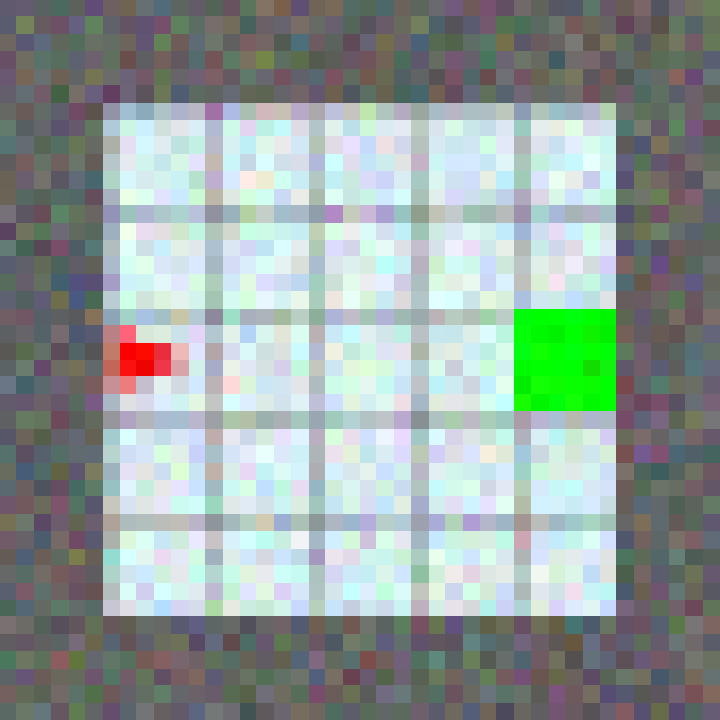
\includegraphics[width=0.49\textwidth]{figures/sec4/MiniGrid-LavaGapS7-v0_observe.pdf}  
        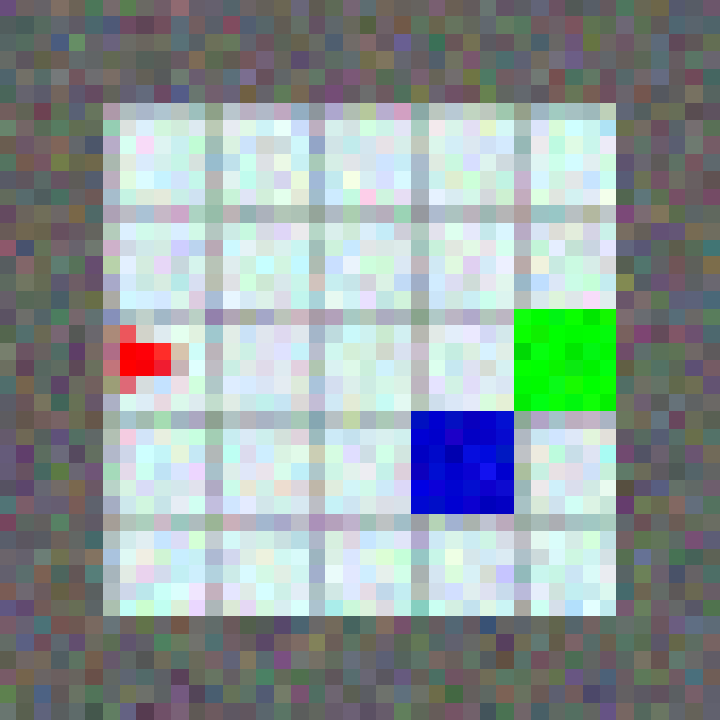
\includegraphics[width=0.49\textwidth]{figures/sec4/MiniGrid-LavaGapS7-v0_full_observe.pdf} 
        \caption{Frozen Lake.}
        \label{fig:gridworld_asym:IceLake:im}
    \end{subfigure}\hfill%
    \begin{subfigure}[t]{0.23\textwidth}  
        
\includegraphics[width=0.49\textwidth]{figures/sec4/MiniGrid-TigerDoorEnv-v0_observe.pdf}
        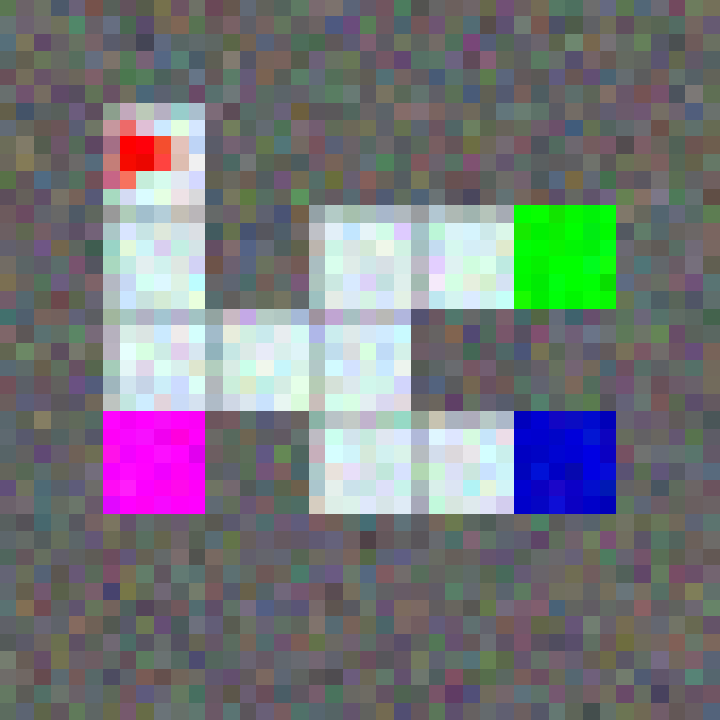
\includegraphics[width=0.49\textwidth]{figures/sec4/MiniGrid-TigerDoorEnv-v0_full_observe.pdf} 
        \caption{Tiger Door.}
        \label{fig:gridworld_asym:TigerDoor:im}
    \end{subfigure}
    \caption{The two gridworlds we study.  An agent (red) must navigate to the goal (green) while avoiding the hazard (blue).  Shown are the raw, noisy $42\times 42$ pixel observations available to the agent.  The expert is conditioned on an omniscient compact state vector indicating the position of the goal and hazard.  In Frozen Lake, the trainee is conditioned on the left image and cannot see the hazard.  In Tiger Door, pushing the button (pink) illuminates the hazard.  } 
    \label{fig:gridworld_asym:grids}
\end{figure}





\section{Failure of Asymmetric Imitation Learning}
\label{sec:il-failure}
We now reason about the failure of AIL in terms of \emph{reward}.  The crucial insight is that to guarantee that the reward earned by the trainee policy is optimal, the divergence between expert and trainee must go to exactly zero.  The reward earned by policies with even a small (but finite) divergence may be arbitrarily low.  This condition, referred to as \emph{identifiability}, is formalized below.  We leverage this condition in Section \ref{sec:algorithm} to derive the update applied to the expert which guarantees the optimal partially observed policy is recovered under the assumptions specified by each theorem, and discussed in further detail in Appendix \ref{supp:thoery}.


\begin{figure*}[t!]
    \centering
    \begin{subfigure}[b]{0.36\textwidth}
        \centering
        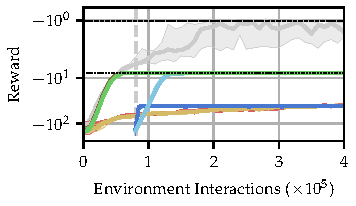
\includegraphics[width=\textwidth]{figures/sec4/cr/lg/sec4_results_IceLake_True_cr_logs_LavaGap_LavaGapCompiledRun_.pdf}
        \caption{Frozen Lake.}
        \label{fig:gridworld_asym:IceLake}
    \end{subfigure}%
    \hfill
    \begin{subfigure}[b]{0.36\textwidth}
        \centering
        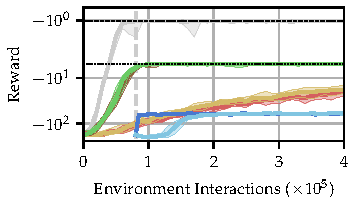
\includegraphics[width=\textwidth]{figures/sec4/cr/td/sec4_results_TigerDoor_True_cr_logs_TigerDoor_TigerDoorCompiledRun_.pdf}
        \caption{Tiger Door.}
        \label{fig:gridworld_asym:TigerDoor}
    \end{subfigure}%
    \hfill
    \begin{subfigure}[b]{0.18\textwidth}
        \centering
       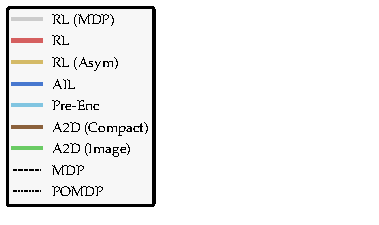
\includegraphics[width=\textwidth]{figures/sec4/legend_sec4_results.pdf}
    \end{subfigure}
    \caption{Results for the gridworld environments.  Median and quartiles across $20$ random seeds are shown.  TRPO~\citep{schulman2015trust} is used for RL methods.  Broken lines indicate the optimal reward, normalized so the optimal MDP reward is $-1$ (\emph{MDP}).  All agents and trainees are conditioned on a image-based input, except \emph{A2D (Compact)} which is conditioned on a partial compact state representation.  All experts, and \emph{RL (MDP)}, are conditioned on an omniscient compact state.  \emph{Pre-Enc} uses a fixed pretrained image encoder, trained on examples from the MDP.  \emph{AIL} and \emph{Pre-Enc} begin when the MDP has converged, as this is the required expenditure for training.  A2D is the only method that reliably and efficiently finds the optimal POMDP policy, and, in a sample budget comparable with \emph{RL (MDP)}.  The convergence of A2D is also similar for \emph{both} image-based (\emph{A2D (Image)}) and compact (\emph{A2D (Compact)}) representations, highlighting that we have effectively subsumed the image perception task.  Configurations, additional results and discussions are included in the appendix.}
    \label{fig:gridworld_asym}
\end{figure*}


However, to first motivate and explore this behavior, we introduce two pedagogical environments, referred to as ``Frozen Lake'' and ``Tiger Door''~\citep{littman1995pomdp,Spaan2012}, illustrated in Figure \ref{fig:gridworld_asym:grids}. Both require an agent to navigate to a goal while avoiding hazards.  The trainee is conditioned on an image of the environment where the hazard is not initially visible. The expert is conditioned on an omniscient compact state vector.  Taking actions, reaching the goal, and hitting the hazard incurs rewards of $-2$, $20$, and $-100$ respectively.  In Frozen Lake, the hazard (weak ice) is in a random location in the interior nine squares.  In Tiger Door, the agent can detour via a button, incurring additional negative reward, to reveal the goal location.

We show results for application of AIL, and comparable RL approaches, to these environments in Figure \ref{fig:gridworld_asym}.  These confirm our intuitions:   RL in the MDP (\emph{RL (MDP)}) is stable and efficient, and proceeds directly to the goal, earning maximum rewards of $10.66$ and $6$.  Direct RL in the POMDP (\emph{RL} and \emph{RL (Asym)}) does not converge to a performant policy in the allocated computational budget.  AIL (\emph{AIL}) converges almost immediately, but, to a trainee that averages over expert actions.  In Frozen Lake, this trainee averages the expert over the location of the weak patch, never circumnavigates the lake, and instead crosses directly, incurring an average reward of $-26.6$.  In Tiger Door, the trainee proceeds directly to a possible goal location without pressing the button, incurring an average reward of $-54$.  Both solutions represent catastrophic failures.  Instead, the trainee should circumnavigate the lake, or, push the button and then proceed to the goal, earning rewards of $4$ and $2$ respectively. 

These results, and insight from Theorem \ref{def:ail}, lead us to define two important properties which provide guarantees on the performance of AIL:
\begin{definition}[Identifiable Policies]
\label{def:consistency_pol} 
Given an MDP-POMDP pair $\left\lbrace \mathcal{M}_{\Theta}, \mathcal{M}_{\Phi} \right\rbrace$, an MDP policy $\pi_{\theta} \in \Pi_{\Theta}$, and POMDP policy $\pi_{\phi} \in \Pi_{\Phi}$, we describe $\{\pi_{\theta}, \pi_{\phi}\}$ as an \textbf{identifiable policy pair} if and only if $\mathbb{E}_{d^{\pi_{\phi}}(s,b)} \left[ \mathbb{KL} \left[ \pi_{\theta}(a | s) || \pi_{\phi}(a | b) \right] \right] = 0$.  
\end{definition}
\begin{definition}[Identifiable Processes]
\label{def:consistency_proc} 
If each optimal MDP policy, $\pi_{\theta^*} \in \Pi_{\Theta^*}$, and the corresponding implicit policy, $\hat{\pi}_{\theta^*} \in \hat{\Pi}_{\Theta^*}$, form an identifiable policy pair, then we define $\{\mathcal{M}_{\Theta}, \mathcal{M}_{\Phi}\}$ as an \textbf{identifiable process pair}.  
\end{definition}
Identifiable policy pairs enforce that the partially observing implicit policy, recovered through application of AIL, can \emph{exactly} reproduce the actions of the fully observing policy.  These policies are therefore guaranteed to incur the same reward.  Identifiable processes then extends this definition, requiring that such an identifiable policy pair exists for all optimal fully observing policies.  Using this definition, we can then show that performing AIL using any optimal fully observing policy on an identifiable process pair is guaranteed to recover an optimal partially observing policy: 
\begin{theorem}[Convergence of AIL]
\label{thm:consistency_conv}
For any identifiable process pair defined over sufficiently expressive policy classes, under exact intermediate updates, the iteration defined by:
\begin{equation}
    \hspace*{-0.1cm} \psi_{k+1} \!= \!\mathop{\argmin}_{\psi \in \Psi} \!\! \mathop{\mathbb{E}}_{d^{\pi_{\psi_k}}(s,b)} \! \left[  \mathbb{KL} \left[ \pi_{\theta^*}(a|s) || \pi_\psi(a|b) \right] \right],
\end{equation}
where $\pi_{\theta^*}$ is an optimal fully observed policy, converges to an optimal partially observed policy, $\pi_{\psi^*}(a|b)$, as $k \tends \infty$.
\end{theorem}
\begin{proof}
See Appendix \ref{supp:thoery}.
\end{proof}
Therefore, identifiability of processes defines a sufficient condition to guarantee that any optimal expert policy provides asymptotically unbiased supervision to the trainee.  If a process pair is identifiable, then AIL recovers the optimal partially observing policy, and garners a reward equal to the fully observing expert. When processes are not identifiable, the divergence between expert and trainee is non-zero, and the \emph{reward} garnered by the trainee can be arbitrarily sub-optimal (as in the gridworlds above).  Unfortunately, identifiability of two processes represents a strong assumption, unlikely to hold in practice. Therefore, we propose an extension that modifies the \emph{expert} on-line, such that the modified expert policy and corresponding implicit policy pair form an identifiable \emph{and} optimal policy pair under partial information. This modification, in turn, guarantees that the expert provides asymptotically correct AIL supervision.

% % \aw{even if the divergence has been minimized within the achievable policy class.}

% However, identifiability of two processes is a fixed property of the processes, and represents a strong condition that is unlikely to hold in general, and hence the performance of AIL cannot be guaranteed.  

% We therefore propose an extension that modifies the \emph{expert} on-line, such that the modified expert policy and corresponding implicit policy pair form an identifiable \emph{and} optimal policy pair (under partial information), thereby guaranteeing that the expert provides asymptotically correct AIL supervision.

% % huge final sentence needs to be broken up.
